\documentclass[pdflatex,11pt]{aghdpl}
% \documentclass{aghdpl}               % przy kompilacji programem latex
% \documentclass[pdflatex,en]{aghdpl}  % praca w języku angielskim
\usepackage[polish]{babel}
\usepackage[utf8]{inputenc}
\usepackage{mathtools}
\usepackage[hidelinks]{hyperref}

% dodatkowe pakiety
\usepackage{enumerate}
\usepackage{listings}
\lstloadlanguages{TeX}

\lstset{
  literate={ą}{{\k{a}}}1
           {ć}{{\'c}}1
           {ę}{{\k{e}}}1
           {ó}{{\'o}}1
           {ń}{{\'n}}1
           {ł}{{\l{}}}1
           {ś}{{\'s}}1
           {ź}{{\'z}}1
           {ż}{{\.z}}1
           {Ą}{{\k{A}}}1
           {Ć}{{\'C}}1
           {Ę}{{\k{E}}}1
           {Ó}{{\'O}}1
           {Ń}{{\'N}}1
           {Ł}{{\L{}}}1
           {Ś}{{\'S}}1
           {Ź}{{\'Z}}1
           {Ż}{{\.Z}}1
}

%---------------------------------------------------------------------------

\author{Ernest Jęczmionek}
\shortauthor{E. Jęczmionek}

\titlePL{Zrównoleglenie algorytmu gradientowej klasteryzacji z użyciem technologii GPU}
\titleEN{GPU based parallelization of Complete Gradient Clustering Algorithm}

\shorttitlePL{GPGPU klasteryzacja gradientowa} % skrócona wersja tytułu jeśli jest bardzo długi
\shorttitleEN{GPGPU gradient clustering}

\thesistypePL{Praca magisterska}
\thesistypeEN{Master of Science Thesis}

\supervisorPL{dr hab. inż Piotr Kowalski}
\supervisorEN{Piotr Kowalski Ph.D}

\date{2019}

\departmentPL{Katedra Informatyki Stosowanej i Fizyki Komputerowej}
\departmentEN{Department of Applied Informatics and Computational Physics}

\facultyPL{Wydział Fizyki i Informatyki Stosowanej}
\facultyEN{Faculty of Physics and Applied Computer Science}

\acknowledgements{Serdecznie dziękuję \dots tu ciąg dalszych podziękowań np. dla promotora, żony, sąsiada itp.}



\setlength{\cftsecnumwidth}{10mm}

%---------------------------------------------------------------------------

\begin{document}

\titlepages

\tableofcontents
\clearpage

\chapter{Przedmowa}
\label{cha:przedmowa}

Analiza skupień (klasteryzacja) jest metodą nienadzorowaną, której zadaniem jest podział zbioru na skupienia (klastry) w taki sposób aby elementy podobne znajdowały się we wspólnym skupieniu, natomiast niepodobne w odzielnych. Do określania miary podobieństwa bądź niepodobieństwa wykorzystuje się rozmaite metryki. Obecnie dzięki rozwojowi usług internetowych, targetowaniu klientów czy segmentacji obrazów zachodzi duże zapotrzebowanie na skuteczne metody analizy skupień.

Wraz z rozwojem technologicznym coraz trudniejsze staje się tworzenie jednostek o większej wydajności pojedynczego rdzenia. Przyczyną tego są bariery fizyczne takie jak proces technologiczny litografii czy moc generowana przez układ za czym podąża problem chłodzenia. Rozwiązaniem tego problemu staje się tworzenie układów o coraz większej liczbie rdzeni. Z czasem zauważono potencjał w kartach graficznych dysponujących obecnie kilkuset krotnie większą liczbą rdzeni w stosunku do procesorów. Pierwszym środowiskiem oferującym programistom łatwy sposób wykorzystania kart graficznych do obliczeń ogólnego przeznaczenia stała się CUDA.
%---------------------------------------------------------------------------

\section{Cele pracy}
\label{sec:celePracy}

Niniejsza praca będzie się skupiała na przyspieszeniu działania algorytmu gradientowej klasteryzacji przy wykorzystaniu akceleratorów graficznych.


%---------------------------------------------------------------------------

\section{Zawartość pracy}
\label{sec:zawartoscPracy}

Zostaną przedstawione popularne metody klasteryzacji oraz algorytm przewodni pracy wraz z jego niedogodnościami. Omówione i porównane będą dwa wiodące środowiska wykorzystujące akceleratory graficzne. Algorytm gradientowej klasteryzacji zostanie zrównoleglony zarówno przy użycie procesora jak i karty graficznej. Porównanie powyższych implementacji posłuży w odpowiedzi na pytanie czy akceleratory graficzne są właściwym rozwiązaniem dla przedstawionej metody klasteryzacji.
\chapter{Wstęp}
\label{cha:wstep}

W tym rozdziale zostaną zaprezentowane metody i technologie konkurencyjne dla tematu tej pracy.

\section{Klasteryzacja}
\label{sec:klasteryzacja}

\subsection{Rys historyczny}
Początki analizy skupień sięgają roku 1932, kiedy to klasteryzacja została opisana w odniesieniu do antropologi \cite{Dri32}, skąd następnie przeniknęła do psychologii. W latach 60-tych nastąpił rozwój eksploracji danych (w tamtym czasie używano nazwy ang.data fishing) na bazie metod statystycznych operujących na stosunkowo niewielkich zbiorach danych. Wzrost dostępności komputerów spowodował olbrzymi wzrost liczności zbiorów, z którymi musiano sobie poradzić. Obecnie analiza skupień jest używana m.in. do rozróżniania tkanek na prześwietleniach, grupowania klientów, znajdywania społeczności, segmentacji obrazów, systemów rekomendacji, detekcji anomalii, lokalizacji miejsc o zagrożeniu pożarowym lub bezpieczeństwa czy śledzenia obiektów.

\subsection{Algorytm k-średnich}
Algorytm k-średnich został wprowadzony przez Jamesa MacQueena \cite{Mac67} na postawie idei żydowskiego matematyka polskiego pochodzenia Hugo Steinshausa z lwowskiej szkoły matematycznej.\newline
Ma on za zadanie przypisać n elementów zbioru do k klastrów, gdzie k jest znane. Jest to problem NP-trudny, dlatego metoda korzysta z heurystyki, a przedstawia się ona następująco:
\begin{enumerate}
	\item{załóż liczbę klastrów k}
	\item{wylosuj środki klastrów $\mu_i$}
	\item{przypisz elementy zbioru do klastrów o najbliższym środku}
	\item{wylicz nowe środki klastrów jako średnie elementów w skupieniu}
	\item{wróć do punktu 3 jeśli nastąpiła zmiana przynależności do klastrów w punkcie 4}
\end{enumerate}
Niestety algorytm posiada kilka wad. Brak determinizmu wynika bezpośredniego z punktu 2, gdzie środki klastrów są losowane. Będzie to wpływać na przynależność szczególnie elementów znajdujących na brzegach klastrów. Kolejne problemy mogą wynikać z różnej liczności klastrów, różnych gęstości czy nieregularnych kształtów. ZDJĘCIA DODATEK A KLASTERYZACJA DODAJ

\subsection{Algorytmy hierarchiczne}
Celem tej grupy jest budowa hierarchicznych klastrów, które można przedstawić za pomocą dendrogramu. Metody z tej kategorii dzielą się na 2 główne grupy:
\begin{itemize}
	\item aglomeracyjne (bottom-up) - każdy element tworzy własny klaster, które to są łączone w wyższych poziomach hierarchii
	\item deglomeracyjne/podziałowe (top-down) - początek stanowi jeden klaster, dzieląc się w miarę schodzenia w poziomach drzewa
\end{itemize}
Głównymi różnicami pomiędzy implementacjami tych metod jest metryka i sposób łączenia. Najpopularniejsza okazała się metoda aglomeracyjna, lecz posiada złożoność czasową $\mathcal{O}(n^3)$ i pamięciową $\mathcal{O}(n^2)$.

\subsection{Algorytmy gęstościowe DBSCAN}
Density-based spatial clustering of applications with noise jest najmłodszym z prezentowanych algorytmów a zarazem jednym z najczęściej cytowanej i najbardziej popularnych \cite{Est96}.
Podstawowe pojęcia:
\begin{itemize}
	\item punkt rdzeniowy (ang. core point) - punkt w otoczeniu $\epsilon$ posiada co najmniej $minPts$
	\item punkt brzegowy (ang. border point) - punkt nie jest rdzeniowy, lecz leży w otoczenie $\epsilon$ punktu rdzeniowego
	\item punkt szumu (ang. noise point) - punkt nie jest rdzeniowy ani brzegowy
\end{itemize}
Abstrakt algorytmu przedstawia się następująco: \cite{Sch17}
\begin{enumerate}
	\item wyznacz sąsiadów dla każdego punktu w otoczeniu $\epsilon$ i oceń czy jest rdzeniowy
	\item złącz punkty rdzeniowe w otoczeniu $\epsilon$ w klastry
	\item dla każdego nierdzeniowego punkty oznacz go jako punkt brzegowy lub punkt szumu
\end{enumerate}
Złożoność czasowa algorytmu w przypadku pesymistycznym wynosi $\mathcal{O}(n^2)$ co jest akceptowalne. Do wad należy zaliczyć niedeterministyczność w klasteryzacji punktów brzegowych, ponieważ przydzielenie ich może zależeć od kolejności ułożenia danych. Dla wielowymiarowych danych metryki odległościowe mogą prowadzić do tzw. "przekleństwa wielowymiarowości" co znacząco utrudnia dobór $\epsilon$, co więcej wybór otoczenia nie jest trywialny gdy brak specjalistycznej wiedzy na temat danych. Dostosowanie minimalnej liczby sąsiadów stanowiącej punkt rdzeniowy jest trudne, gdy klastry znacząco różnią się gęstością.

\subsection{Sposoby oceny klasteryzacji}
INDEKS RANDA, CLUSTER COHESION, CLUSTER SEPARATION, DAVIES-BOULDIN, DUNN

\section{Akceleracja GPU}
\label{sec:akceleracja}
\chapter{Algorytm gradientowej klasteryzacji}
\label{cha:gradient_clustering_algorithm}

\section{Estymatory jądrowe}
\label{sec:estymatory}
\subsection{Definicja}

Niech zmienna losowa $X$ będzie n-wymiarową zmienną losową o gęstości prawdopodobieństwa $f$. Estymator tej zmiennej będzie wyzanoczony na podstawie próby losowej
\begin{equation}
x_1, x_2, ..., x_m
\end{equation}
będacej interpretowaną jako doświadczenie z niezależnych eksperymentów zmiennej losowej $X$.
Jądrowy estymator gęstości $\hat{f}: \mathbf{R} \to [0, \infty)$ dany jest wzorem
\begin{equation}
\label{eq:estymator}
\hat{f}(x)=\frac{1}{mh^n} \displaystyle \sum_{i=1}^{m}K(\frac{x-x_i}{h})
\end{equation}
$m \in \mathbf{N_+}$ jest licznością próby losowej, $h \in \mathbf{R_+}$ jest parametrem wygładzania, a funkcja $K$ jest jądrem spełniającym warunki: \\
gęstość funkcji jest znormalizowana
\begin{equation}
\int_{\mathbf{R^n}} K(x)dx = 1
\end{equation}
funkcja jest symetryczna
\begin{equation}
K(x) = K(-x)
\end{equation}
ma w zerze maksimum globalne
\begin{equation}
K(0) \geq K(x), x \in \mathbf{R^n}
\end{equation}

\subsection{Wybór jądra}
Czy pisać o tym?

\subsection{Błąd estymacji}
MSE(ang. mean square error), czyli błąd średniokwadratowy jest kwadratem błędu estymacji, co można zapisać jako
\begin{equation}
MSE = E({(\hat{b}-b)}^2 )
\end{equation}
Wzór można przekształcić w bardziej dogodną formę
\begin{equation}
MSE = {[E(\hat{b})-b]}^2 +V(\hat{b})
\end{equation}
jako sumę kwadratu obciążenia i jego wariancji. Pierwszy człon wskazuje odchylenie "centrów" estymatora z wartościami pomiarowymi, natomiat drugi pokazuje odchylenie względem "centrum". \\
Dla estymatora gęstości prawdopodobieństwa zmiennej n-wymiarowej wzór przyjmuje postać
\begin{equation}
MSE_x = E({[\hat{f}(x)-f(x)]}^2), x \in \mathbf{R^n}
\end{equation}
lub jak poprzednio
\begin{equation}
MSE_x = {[E(\hat{f}(x))-f(x)]}^2 + V(\hat{f}(x)), x \in \mathbf{R^n}
\end{equation}

MISE(ang. mean integrated square error), czyli scałkowany błąd średniokwadratowy otrzymuje się poprzez scałkowanie poprzednich błędów na przestrzeni $\mathbf{R^n}$:
\begin{equation}
MISE = \int_{\mathbf{R^n}} E({[\hat{f}(x)-f(x)]}^2) dx
\end{equation}
lub
\begin{equation}
\label{eq:mise}
MISE = \int_{\mathbf{R^n}} [{[E(\hat{f}(x))-f(x)]}^2 + V(\hat{f}(x))]dx
\end{equation}

Wzór \eqref{eq:mise} podobnie jak poprzednio jest sumą scałkowanego obciążenia estymatora $\hat{f}$ i jego wariancji. MISE jest cennym kryterium dla wyboru postaci jądra $K$ oraz parametru wygładzania $h$.

CZY CIĄGNĄĆ DALEJ? 

\subsection{Parametr wygładzania}

Wartość parametru wygładzania ma kluczowe znaczenie dla jakości estymatora jądrowego. W tym podrozdziale zostaną przedstawione dwie metody wyznaczania tego parametru, przy użyciu MISE - scałkowanego błędu średniokwardatowego. Parametr wygładzania wpływa jednakowo na wszystkie wymiary, w następnym podrozdziale zostanie omówiana metoda jego indywidualizacji w zależności od wymiaru UWAGA ZASTANÓW SIĘ CO PISZESZ \ref{subsec:modyfikacje_h}.

W przypadku gdy zmienna losowa X jest wielowymiarowa wartość parametru wygładzania jest wyliczana osobno dla każdego wymiaru jak dla zmiennych jednowymiarowych. 

W odróżnieniu od problemu wyboru jądra dobór odpowiedniego parametru wygładzania ma kluczowe znaczenie dla jakości estymacji. Jego zbyt mała wartość skutkuje powstaniem wielu ekstemów lokalnych nie mających odzwierciedlenia w danych pomiarowych. Można to również zaobserwować ze wzoru na estymator jądrowy \ref{eq:estymator}, w którym parametr wygładzania znajduje się w mianowniku przed sumą. W takiej sytuacji wzmacnione zostaną wartości znajdujące się blisko "centrum", natomiast bardziej odległe zostaną wytłumione.

W przeciwnym przypadku, gdy omawiany parametr zostanie dobrany zbyt duży doprowadzi to do nadmiernego wygładzenia estymatora. Stłumienie "centrum" i wzmocnienie "ogonów" spowoduję zanik cech danych pomiarowych, uniemożliwiając ich odróżnienie.

DODAJ RYSUNKI dla h małe, duże i OK

INTERPRETACJA 2 z obciążeniem i wariancją





\subsection{Modyfikacja parametru wygładzania}
\label{subsec:modyfikacje_h}

\subsection{Liczność próby losowej}

\subsection{Przykład}



TEST CYTATÓW
\cite{Kul10}
\cite{Kul05}
\cite{Kul12}

\chapter{CUDA}
\label{cha:cuda}

\section{Opis środowiska}
\label{sec:opis_cuda}

\section{Implementacja}
\label{sec:implementacja}


\appendix
\chapter{Dodatki}
\label{cha:dodatekKlasteryzacja}

\section{k-średnich}
\label{sec:k_means}

\begin{figure}[h]
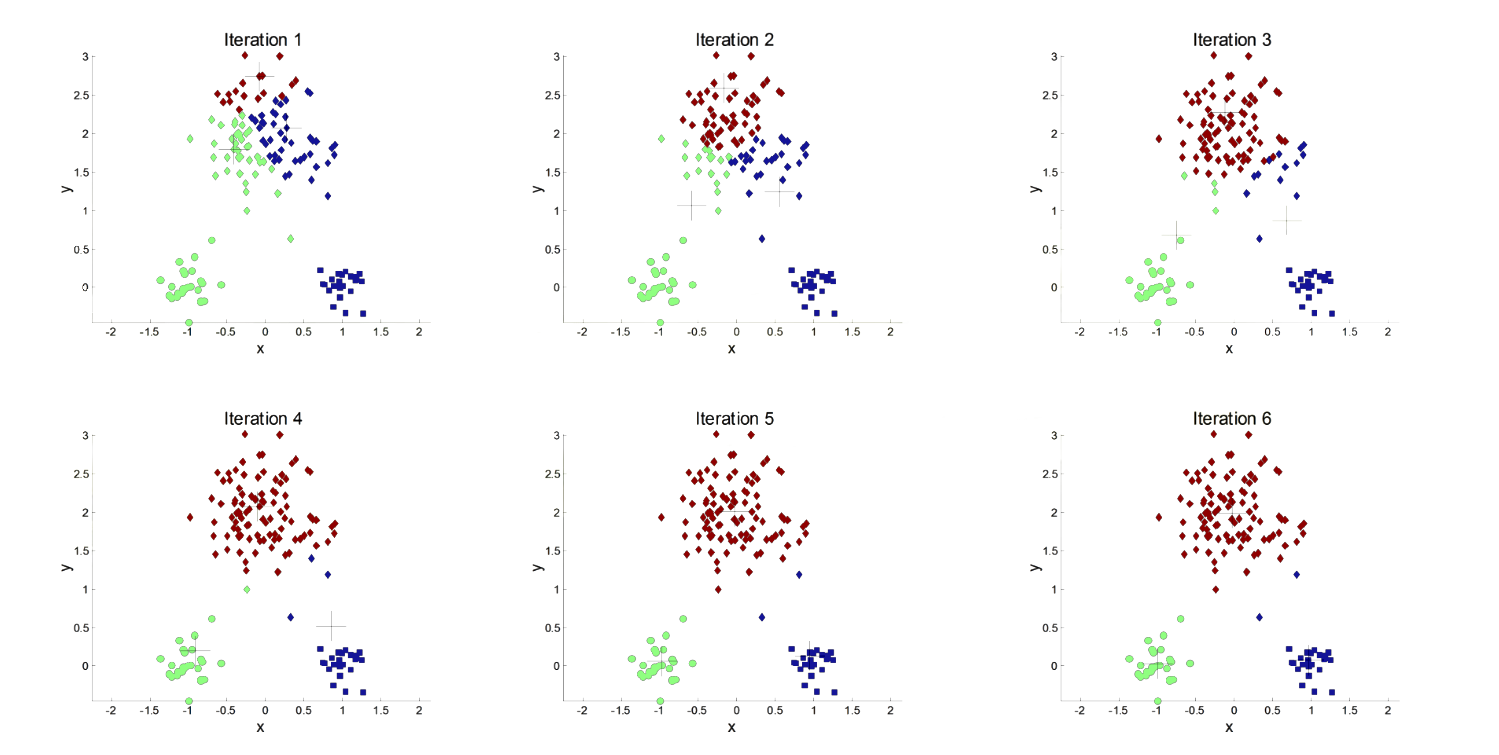
\includegraphics[width=\textwidth]{img/kmeans_startA}
\caption{Warunki początkowe A \cite{Luk}}
\end{figure}

\begin{figure}[H]
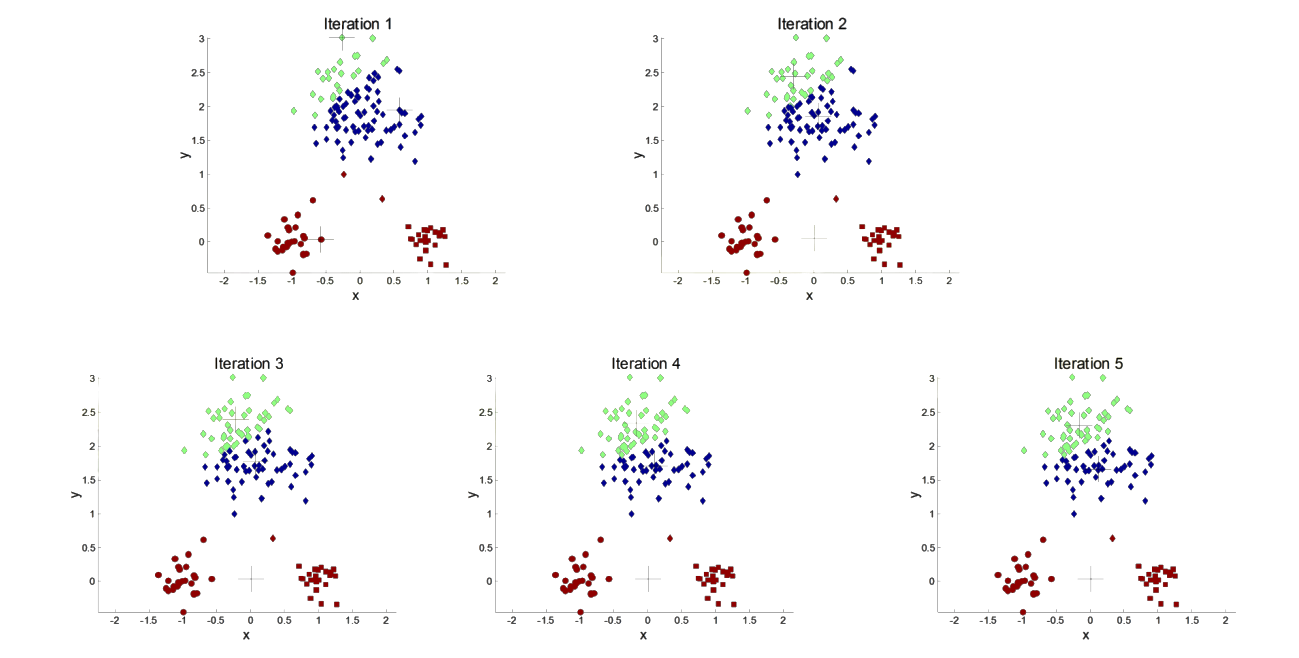
\includegraphics[width=\textwidth]{img/kmeans_startB}
\caption{Warunki początkowe B \cite{Luk}}
\end{figure}

\begin{figure}[H]
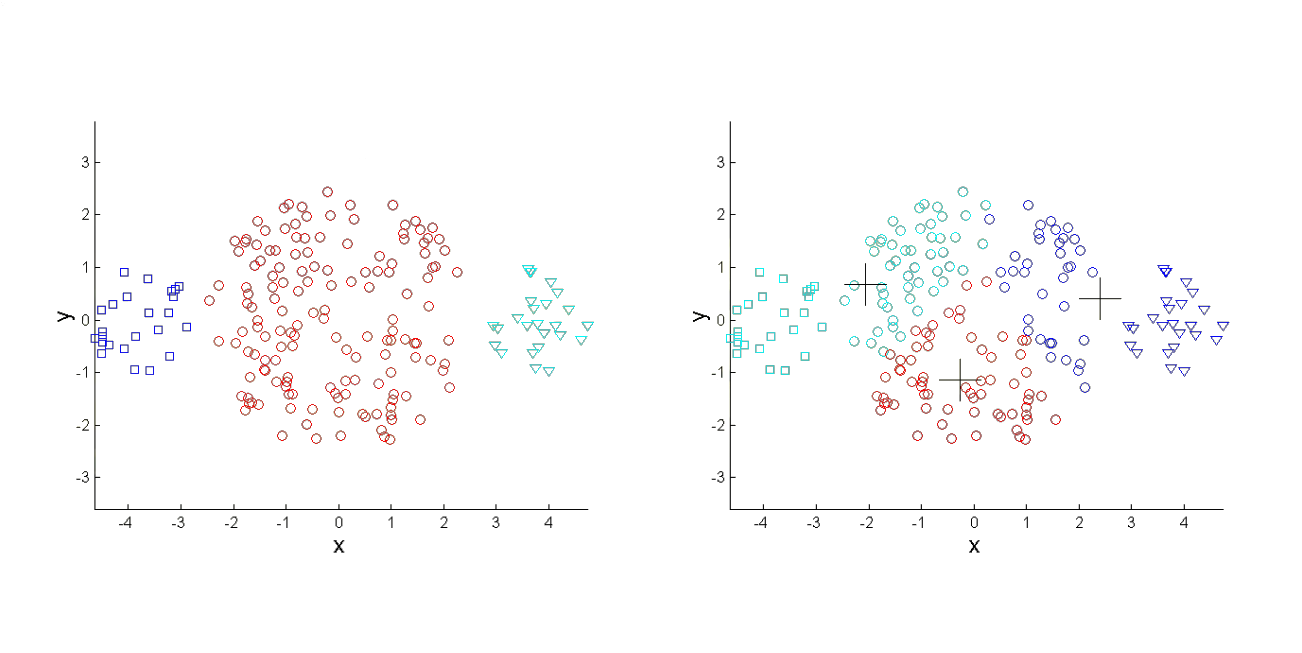
\includegraphics[width=\textwidth]{img/kmeans_quantity}
\caption{Różne liczności klastrów \cite{Luk}}
\end{figure}

\begin{figure}[H]
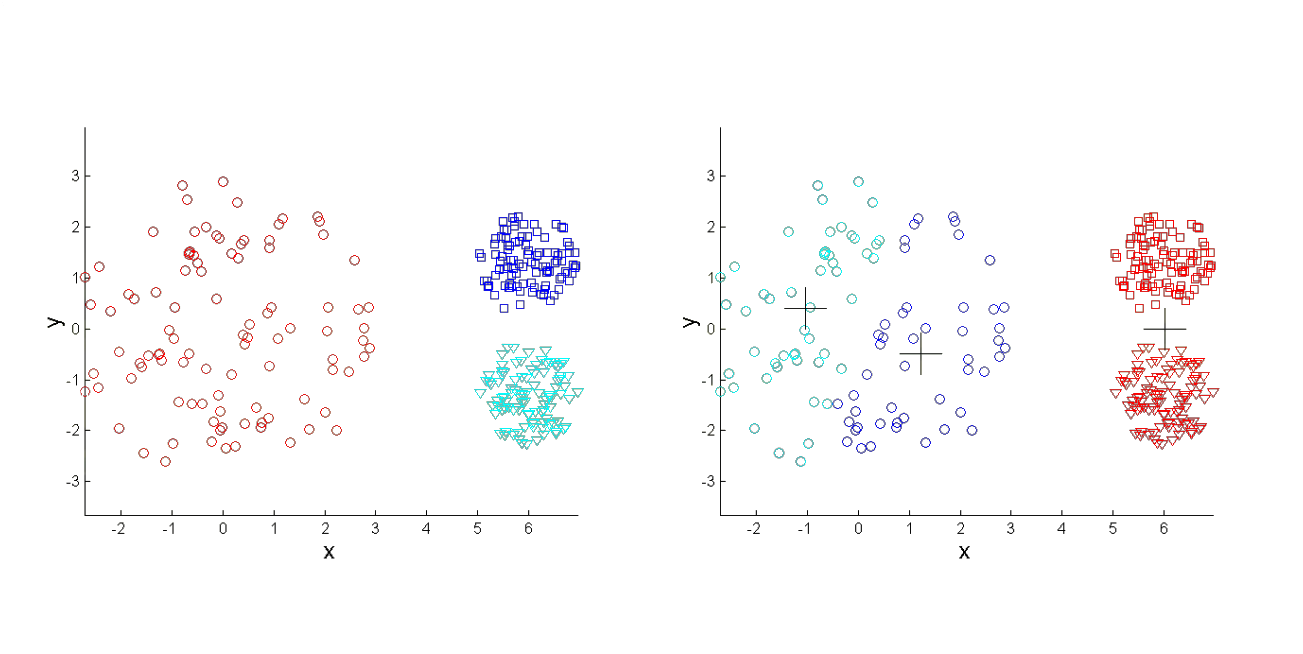
\includegraphics[width=\textwidth]{img/kmeans_density}
\caption{Różne gęstości klastrów \cite{Luk}}
\end{figure}

\begin{figure}[H]
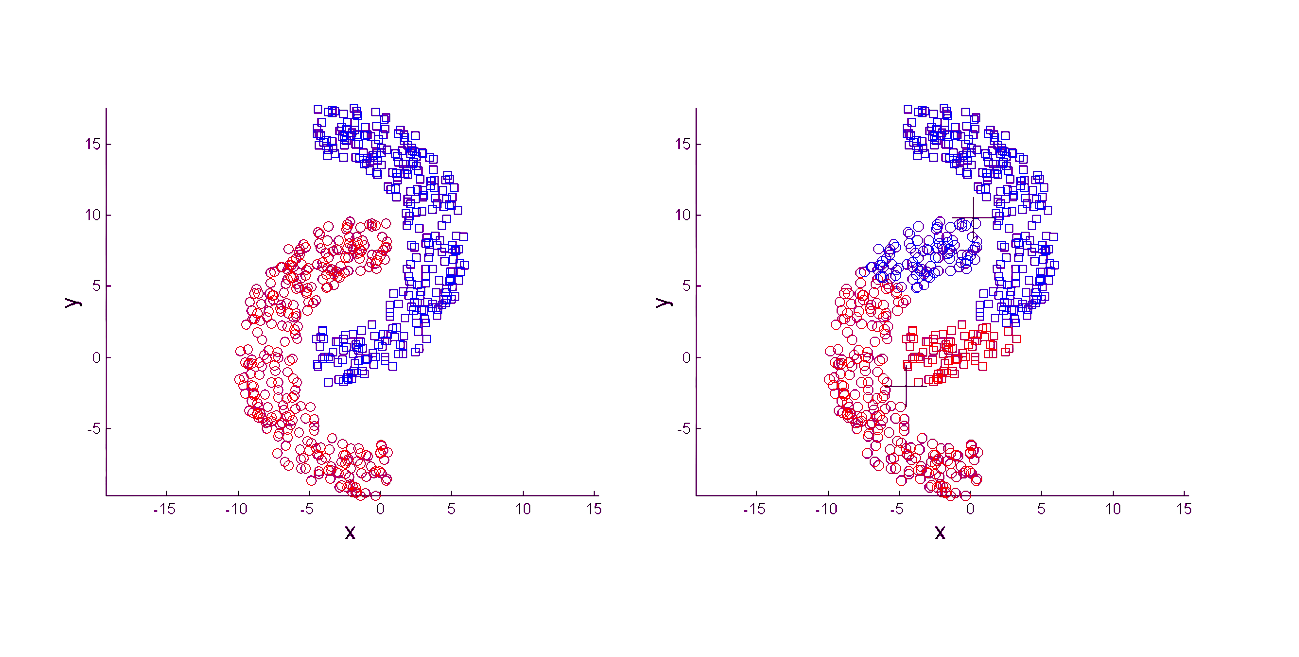
\includegraphics[width=\textwidth]{img/kmeans_irregular}
\caption{Nieregularne kształty klastrów \cite{Luk}} 
\end{figure}

\section{Parametr wygładzania - przykład}
\label{sec:dod_h}

\begin{figure}[H]
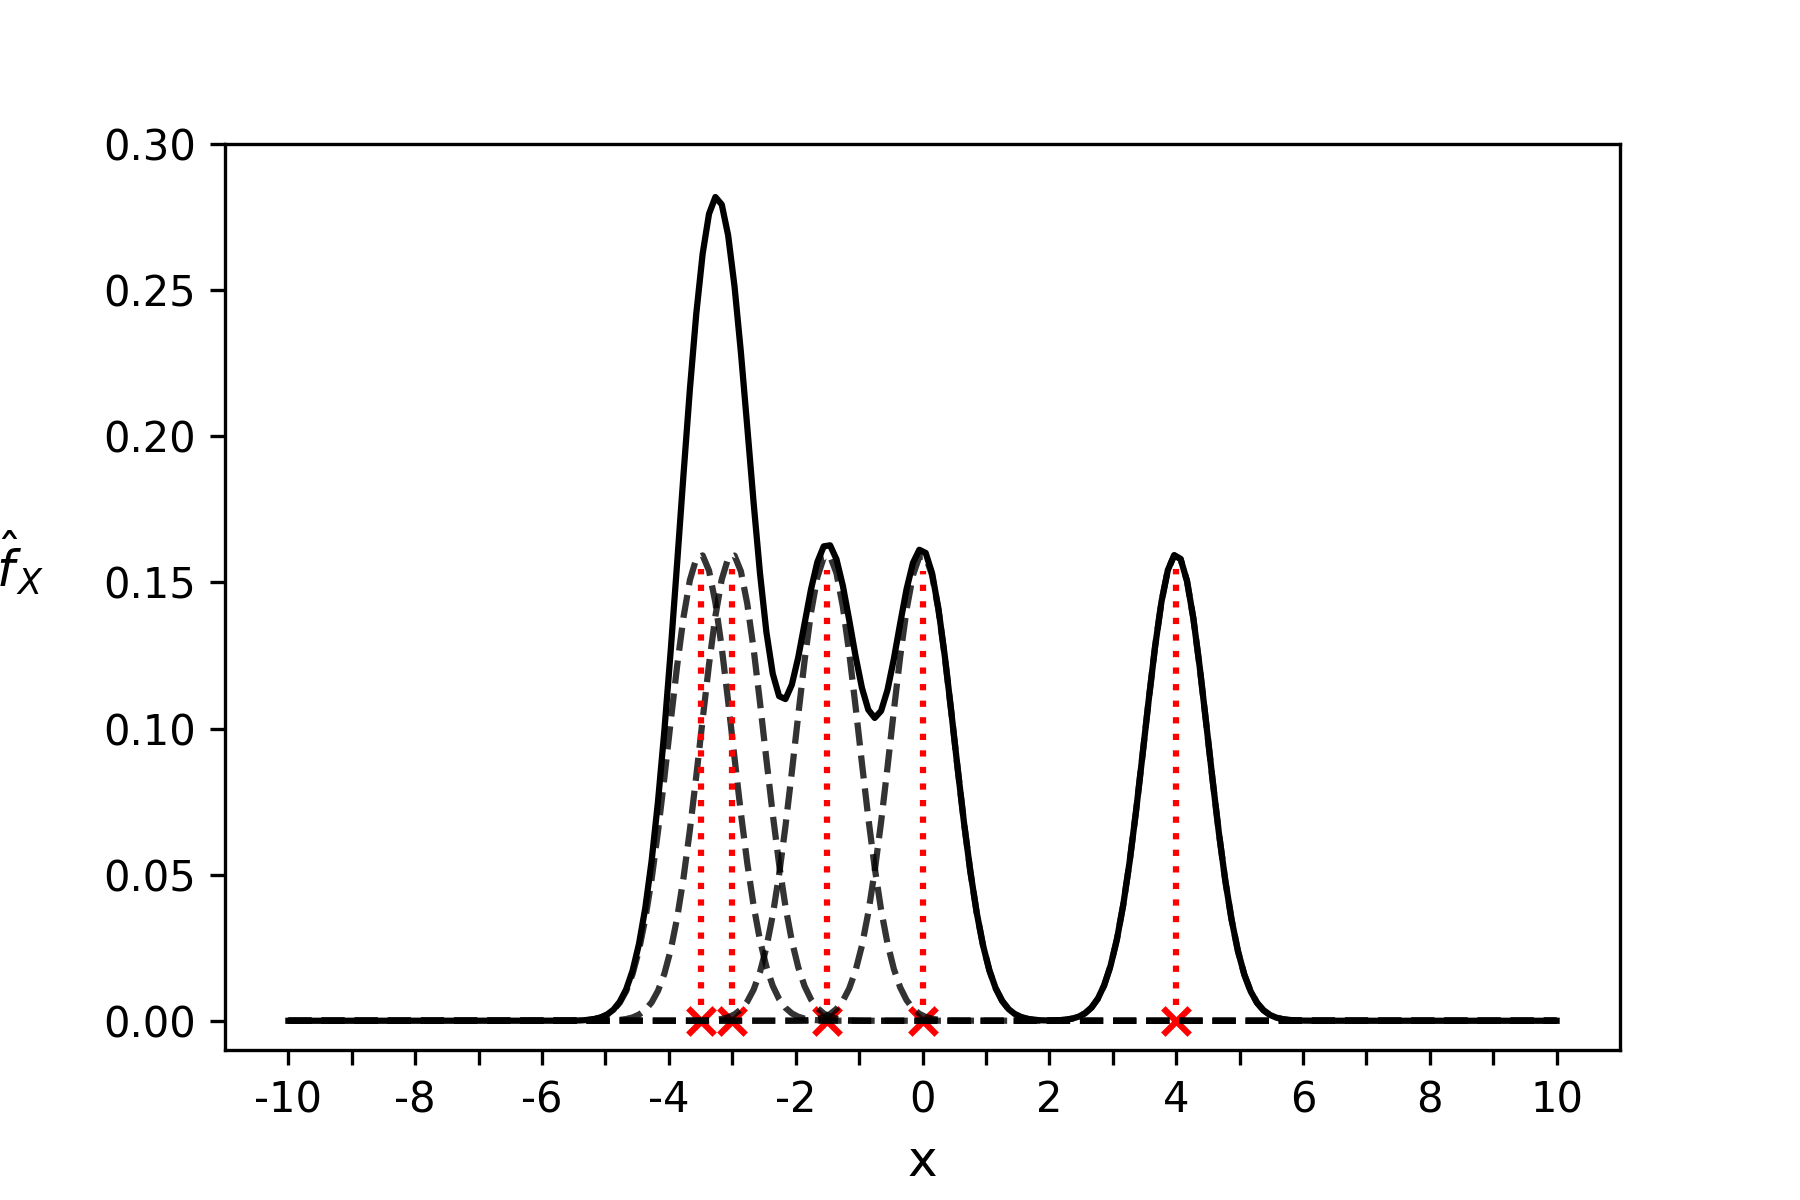
\includegraphics[width=0.9\textwidth]{img/h_05}
\caption{$h=0.5$ \cite{Fra}}
\end{figure}

\begin{figure}[H]
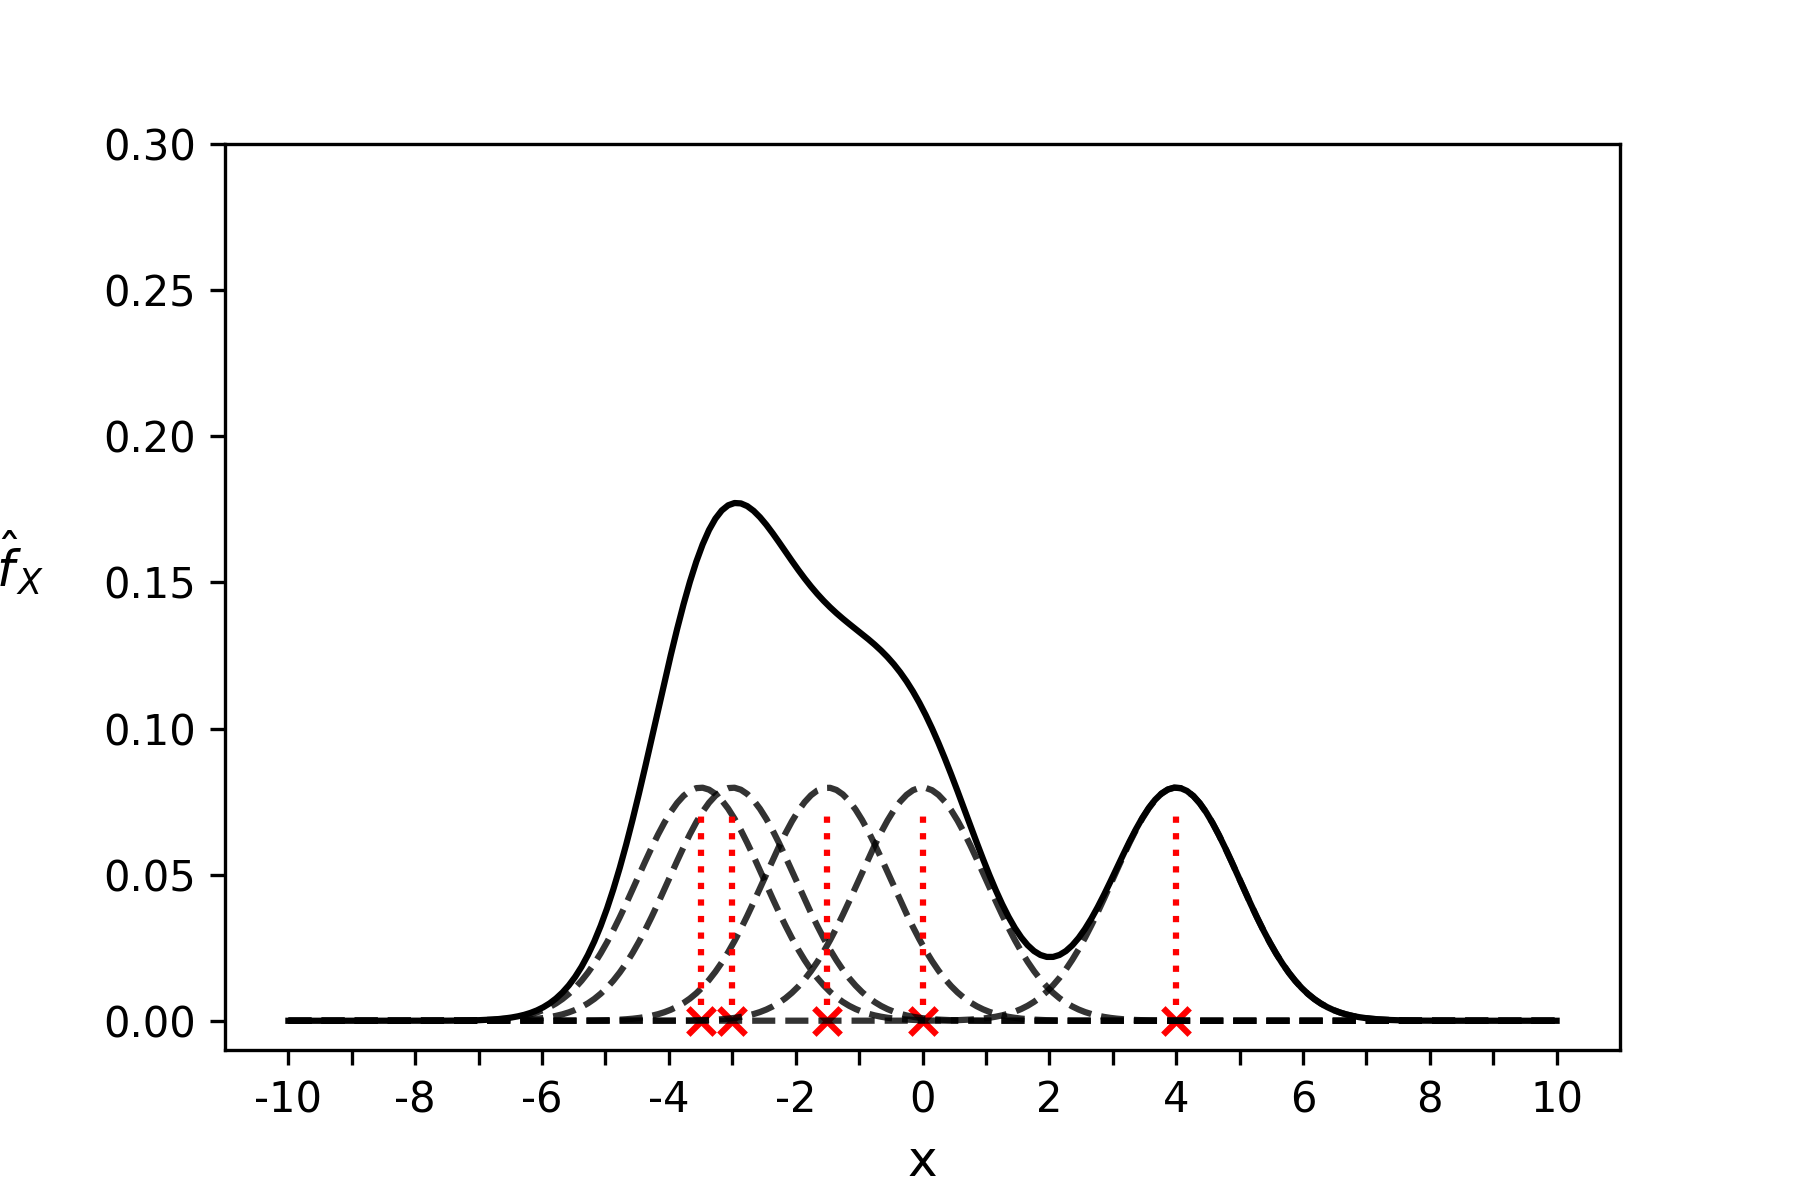
\includegraphics[width=0.9\textwidth]{img/h_1}
\caption{$h=1$ \cite{Fra}}
\end{figure}

\begin{figure}[H]
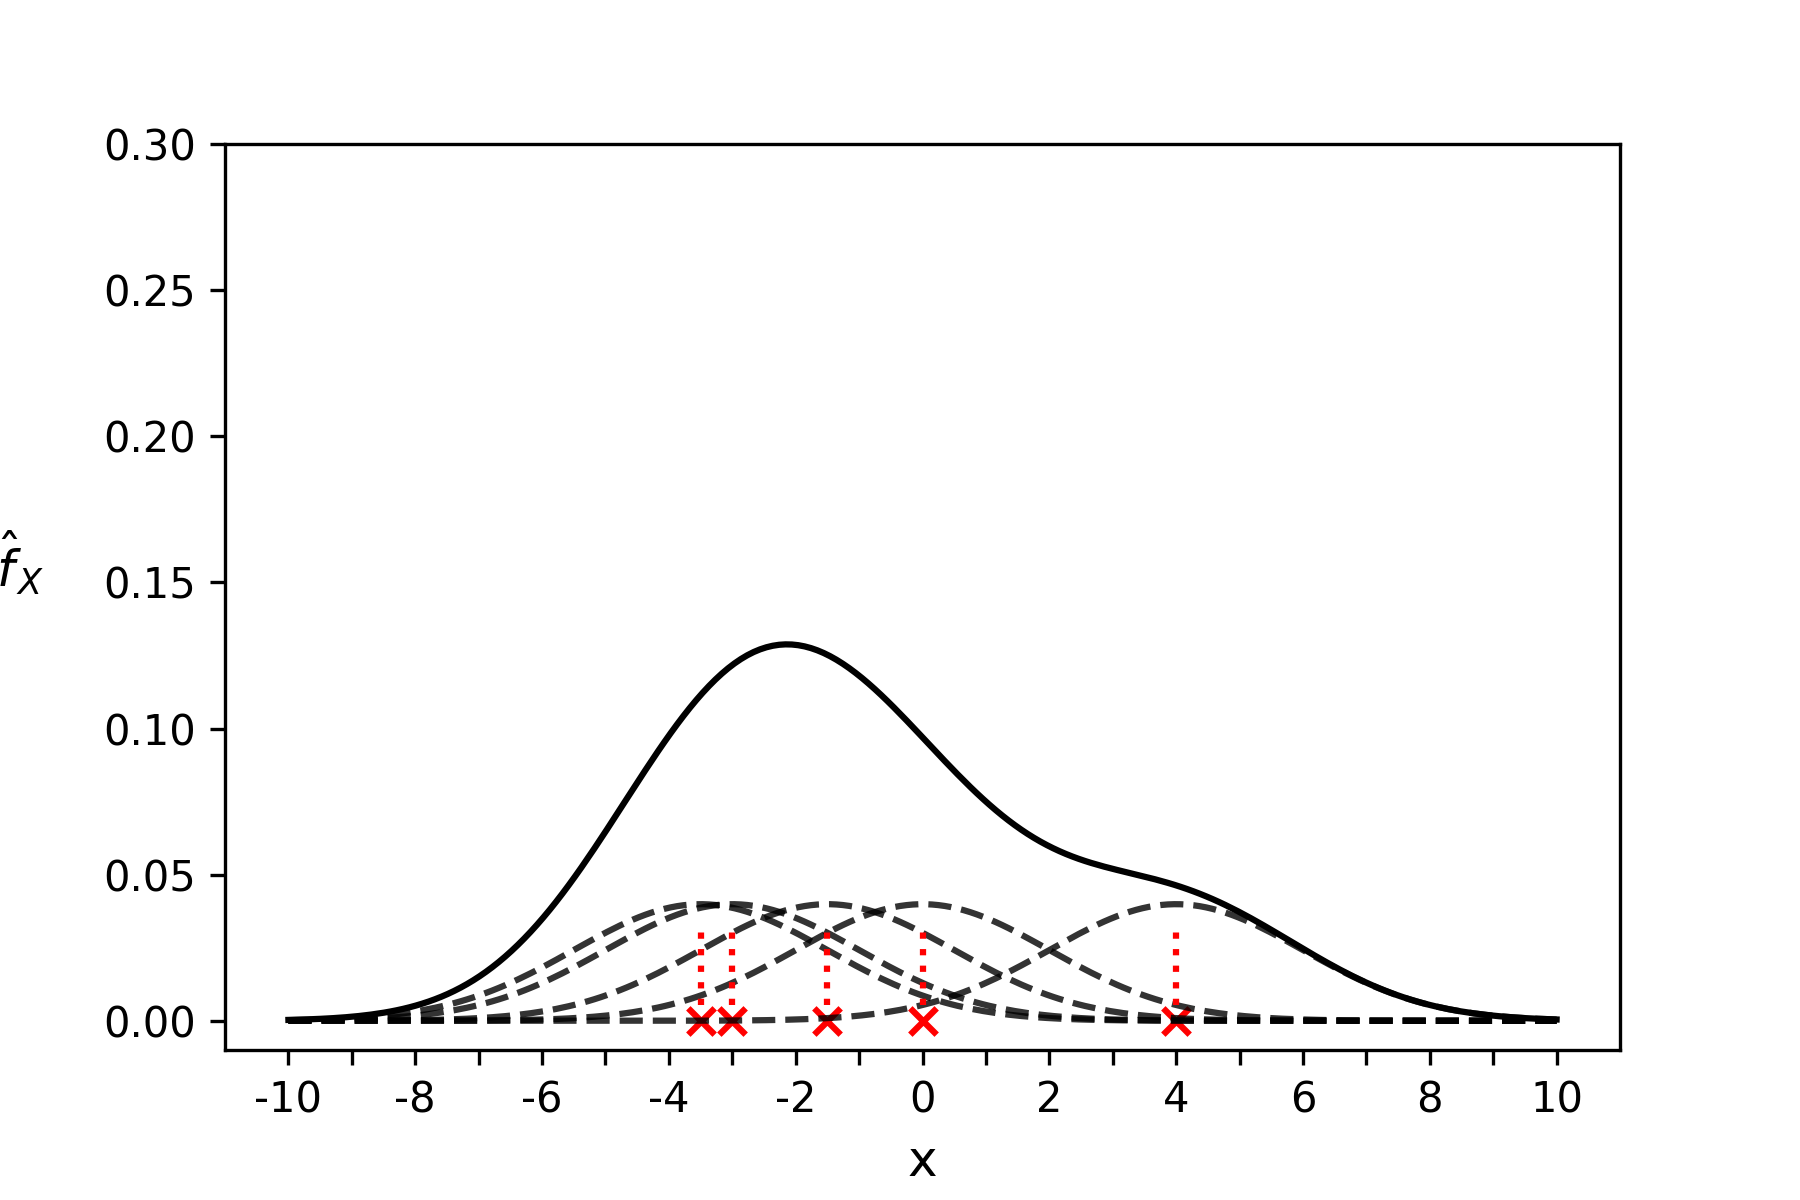
\includegraphics[width=0.9\textwidth]{img/h_2}
\caption{$h=2$ \cite{Fra}}
\end{figure}

\section{Metoda złotego podziału}
\label{sec:dod_gold_ratio}
\begin{table}[H]
\resizebox{\textwidth}{!}{%
\begin{tabular}{|c|c|c|c|c|c|c|c|}
\hline
\multicolumn{4}{|c|}{\textbf{CPU}}                      & \multicolumn{4}{c|}{\textbf{GPU}}                       \\ \hline
\textbf{l} & \textbf{f(l)} & \textbf{r} & \textbf{f(r)} & \textbf{l} & \textbf{f(l)} & \textbf{r} & \textbf{f(r)} \\ \hline
3819.66    & -0.000131275  & 6180.34    & -8.11E-05     & 3819.66    & -0.000135024  & 6180.34    & -8.34E-05     \\ \hline
2360.68    & -0.000212407  & 3819.66    & -0.000131275  & 2360.68    & -0.000218474  & 3819.66    & -0.000135024  \\ \hline
1458.98    & -0.000343682  & 2360.68    & -0.000212407  & 1458.98    & -0.000353498  & 2360.68    & -0.000218474  \\ \hline
901.7      & -0.000556089  & 1458.98    & -0.000343682  & 901.7      & -0.000571971  & 1458.98    & -0.000353498  \\ \hline
557.281    & -0.000899771  & 901.7      & -0.000556089  & 557.281    & -0.000925467  & 901.7      & -0.000571971  \\ \hline
344.419    & -0.00145586   & 557.281    & -0.000899771  & 344.419    & -0.0014974    & 557.281    & -0.000925467  \\ \hline
212.862    & -0.00235551   & 344.419    & -0.00145586   & 212.862    & -0.00242268   & 344.419    & -0.0014974    \\ \hline
131.556    & -0.00380968   & 212.863    & -0.00235551   & 131.556    & -0.00391946   & 212.863    & -0.00242268   \\ \hline
81.3063    & -0.00616118   & 131.556    & -0.00380968   & 81.3063    & -0.00633975   & 131.556    & -0.00391946   \\ \hline
50.2501    & -0.00996563   & 81.3063    & -0.00616118   & 50.2501    & -0.0102493    & 81.3063    & -0.00633975   \\ \hline
31.0563    & -0.01612      & 50.2501    & -0.00996563   & 31.0563    & -0.0165477    & 50.2501    & -0.0102493    \\ \hline
19.1939    & -0.0260727    & 31.0563    & -0.01612      & 19.1939    & -0.0266236    & 31.0563    & -0.0165477    \\ \hline
11.8625    & -0.0421322    & 19.1939    & -0.0260727    & 11.8625    & -0.042452     & 19.1939    & -0.0266236    \\ \hline
7.33148    & -0.0674266    & 11.8625    & -0.0421322    & 7.33148    & -0.0661855    & 11.8625    & -0.042452     \\ \hline
4.53114    & -0.10196      & 7.33148    & -0.0674266    & 4.53114    & -0.0979095    & 7.33148    & -0.0661855    \\ \hline
2.80044    & -0.132709     & 4.53114    & -0.10196      & 2.80044    & -0.13074      & 4.53114    & -0.0979095    \\ \hline
1.7308     & -0.154332     & 2.80044    & -0.132709     & 1.7308     & -0.153345     & 2.80044    & -0.13074      \\ \hline
1.06973    & -0.172337     & 1.7308     & -0.154332     & 1.06973    & -0.168699     & 1.7308     & -0.153345     \\ \hline
0.66117    & -0.188525     & 1.06973    & -0.172337     & 0.66117    & -0.184043     & 1.06973    & -0.168699     \\ \hline
0.408664   & -0.19887      & 0.66117    & -0.188525     & 0.408664   & -0.194777     & 0.66117    & -0.184043     \\ \hline
0.252606   & -0.202492     & 0.408664   & -0.19887      & 0.252606   & -0.199544     & 0.408664   & -0.194777     \\ \hline
0.156157   & -0.201241     & 0.252606   & -0.202492     & 0.156157   & -0.201232     & 0.252606   & -0.199544     \\ \hline
0.252606   & -0.202492     & 0.312215   & -0.201655     & 0.0965488  & -0.20166      & 0.156157   & -0.201232     \\ \hline
0.215766   & -0.202399     & 0.252606   & -0.202492     & 0.0597086  & -0.201579     & 0.0965488  & -0.20166      \\ \hline
0.252606   & -0.202492     & 0.275375   & -0.202229     & 0.0965488  & -0.20166      & 0.119317   & -0.201562     \\ \hline
0.238535   & -0.202504     & 0.252606   & -0.202492     & 0.0824771  & -0.201672     & 0.0965488  & -0.20166      \\ \hline
0.229838   & -0.202477     & 0.238535   & -0.202504     & 0.0737803  & -0.201656     & 0.0824771  & -0.201672     \\ \hline
0.238535   & -0.202504     & 0.243909   & -0.202501     & 0.0824771  & -0.201672     & 0.087852   & -0.201672     \\ \hline
0.235213   & -0.2025       & 0.238535   & -0.202504     & 0.087852   & -0.201672     & 0.0911739  & -0.201669     \\ \hline
0.238535   & -0.202504     & 0.240588   & -0.202496     & 0.085799   & -0.201673     & 0.087852   & -0.201672     \\ \hline
0.237266   & -0.202491     & 0.238535   & -0.202504     & 0.0845302  & -0.201673     & 0.085799   & -0.201673     \\ \hline
0.238535   & -0.202504     & 0.239319   & -0.202498     & 0.085799   & -0.201673     & 0.0865832  & -0.201673     \\ \hline
0.23805    & -0.202489     & 0.238535   & -0.202504     & 0.0853143  & -0.201673     & 0.085799   & -0.201673     \\ \hline
0.238535   & -0.202504     & 0.238834   & -0.2025       & 0.085799   & -0.201673     & 0.0860985  & -0.201673     \\ \hline
\end{tabular}%
}
\caption{Metoda złotego podziału - irys 150 elementów}
\end{table}

\begin{table}[H]
\resizebox{\textwidth}{!}{%
\begin{tabular}{|c|c|c|c|c|c|c|c|}
\hline
\multicolumn{4}{|c|}{\textbf{CPU}}                      & \multicolumn{4}{c|}{\textbf{GPU}}                       \\ \hline
\textbf{l} & \textbf{f(l)} & \textbf{r} & \textbf{f(r)} & \textbf{l} & \textbf{f(l)} & \textbf{r} & \textbf{f(r)} \\ \hline
3819.66   & -0.000132857 & 6180.34   & -8.21E-05    & 3819.66   & -0.000134994 & 6180.34   & -8.34E-05    \\ \hline
2360.68   & -0.000214967 & 3819.66   & -0.000132857 & 2360.68   & -0.000218425 & 3819.66   & -0.000134994 \\ \hline
1458.98   & -0.000347823 & 2360.68   & -0.000214967 & 1458.98   & -0.000353419 & 2360.68   & -0.000218425 \\ \hline
901.7     & -0.00056279  & 1458.98   & -0.000347823 & 901.7     & -0.000571845 & 1458.98   & -0.000353419 \\ \hline
557.281   & -0.000910613 & 901.7     & -0.00056279  & 557.281   & -0.000925257 & 901.7     & -0.000571845 \\ \hline
344.419   & -0.0014734   & 557.281   & -0.000910613 & 344.419   & -0.00149707  & 557.281   & -0.000925257 \\ \hline
212.862   & -0.00238402  & 344.419   & -0.0014734   & 212.862   & -0.00242224  & 344.419   & -0.00149707  \\ \hline
131.556   & -0.00385268  & 212.863   & -0.00238402  & 131.556   & -0.00391895  & 212.863   & -0.00242224  \\ \hline
81.3063   & -0.00621678  & 131.556   & -0.00385268  & 81.3063   & -0.00633965  & 131.556   & -0.00391895  \\ \hline
50.2501   & -0.0100459   & 81.3063   & -0.00621678  & 50.2501   & -0.0102521   & 81.3063   & -0.00633965  \\ \hline
31.0563   & -0.0162338   & 50.2501   & -0.0100459   & 31.0563   & -0.0165643   & 50.2501   & -0.0102521   \\ \hline
19.1939   & -0.02622     & 31.0563   & -0.0162338   & 19.1939   & -0.0267006   & 31.0563   & -0.0165643   \\ \hline
11.8625   & -0.0423081   & 19.1939   & -0.02622     & 11.8625   & -0.0427806   & 19.1939   & -0.0267006   \\ \hline
7.33148   & -0.0673237   & 11.8625   & -0.0423081   & 7.33148   & -0.0674937   & 11.8625   & -0.0427806   \\ \hline
4.53114   & -0.101842    & 7.33148   & -0.0673237   & 4.53114   & -0.102513    & 7.33148   & -0.0674937   \\ \hline
2.80044   & -0.142588    & 4.53114   & -0.101842    & 2.80044   & -0.143185    & 4.53114   & -0.102513    \\ \hline
1.7308    & -0.174502    & 2.80044   & -0.142588    & 1.7308    & -0.175082    & 2.80044   & -0.143185    \\ \hline
1.06973   & -0.201401    & 1.7308    & -0.174502    & 1.06973   & -0.201328    & 1.7308    & -0.175082    \\ \hline
0.66117   & -0.243325    & 1.06973   & -0.201401    & 0.66117   & -0.243223    & 1.06973   & -0.201328    \\ \hline
0.408664  & -0.278122    & 0.66117   & -0.243325    & 0.408664  & -0.27807     & 0.66117   & -0.243223    \\ \hline
0.252606  & -0.294904    & 0.408664  & -0.278122    & 0.252606  & -0.294612    & 0.408664  & -0.27807     \\ \hline
0.156157  & -0.301022    & 0.252606  & -0.294904    & 0.156157  & -0.300686    & 0.252606  & -0.294612    \\ \hline
0.0965488 & -0.302597    & 0.156157  & -0.301022    & 0.0965488 & -0.302285    & 0.156157  & -0.300686    \\ \hline
0.0597086 & -0.302554    & 0.0965488 & -0.302597    & 0.0597086 & -0.302338    & 0.0965488 & -0.302285    \\ \hline
0.0965488 & -0.302597    & 0.119317  & -0.302222    & 0.0369402 & -0.302014    & 0.0597086 & -0.302338    \\ \hline
0.0824771 & -0.302682    & 0.0965488 & -0.302597    & 0.0597086 & -0.302338    & 0.0737803 & -0.302412    \\ \hline
0.0737803 & -0.302666    & 0.0824771 & -0.302682    & 0.0737803 & -0.302412    & 0.0824771 & -0.302398    \\ \hline
0.0824771 & -0.302682    & 0.087852  & -0.302672    & 0.0684054 & -0.302398    & 0.0737803 & -0.302412    \\ \hline
0.0791552 & -0.302684    & 0.0824771 & -0.302682    & 0.0737803 & -0.302412    & 0.0771022 & -0.302412    \\ \hline
0.0771022 & -0.302683    & 0.0791552 & -0.302684    & 0.0717273 & -0.302409    & 0.0737803 & -0.302412    \\ \hline
0.0791552 & -0.302684    & 0.0804241 & -0.302687    & 0.0737803 & -0.302412    & 0.0750492 & -0.302413    \\ \hline
0.0804241 & -0.302687    & 0.0812083 & -0.302683    & 0.0750492 & -0.302413    & 0.0758334 & -0.302413    \\ \hline
0.0799394 & -0.302687    & 0.0804241 & -0.302687    & 0.0758334 & -0.302413    & 0.076318  & -0.302412    \\ \hline
0.0796399 & -0.302686    & 0.0799394 & -0.302687    & 0.0755338 & -0.302413    & 0.0758334 & -0.302413    \\ \hline
\end{tabular}%
}
\caption{Metoda złotego podziału - irys 100 elementów}
\end{table}

\begin{table}[H]
\resizebox{\textwidth}{!}{%
\begin{tabular}{|c|c|c|c|c|c|c|c|}
\hline
\multicolumn{4}{|c|}{\textbf{CPU}}                      & \multicolumn{4}{c|}{\textbf{GPU}}                       \\ \hline
\textbf{l} & \textbf{f(l)} & \textbf{r} & \textbf{f(r)} & \textbf{l} & \textbf{f(l)} & \textbf{r} & \textbf{f(r)} \\ \hline
3819.66   & -0.000134824 & 6180.34  & -8.33E-05    & 3819.66   & -0.000134865 & 6180.34  & -8.34E-05    \\ \hline
2360.68   & -0.00021815  & 3819.66  & -0.000134824 & 2360.68   & -0.000218216 & 3819.66  & -0.000134865 \\ \hline
1458.98   & -0.000352974 & 2360.68  & -0.00021815  & 1458.98   & -0.000353081 & 2360.68  & -0.000218216 \\ \hline
901.7     & -0.000571124 & 1458.98  & -0.000352974 & 901.7     & -0.000571295 & 1458.98  & -0.000353081 \\ \hline
557.281   & -0.000924097 & 901.7    & -0.000571124 & 557.281   & -0.000924372 & 901.7    & -0.000571295 \\ \hline
344.419   & -0.00149522  & 557.281  & -0.000924097 & 344.419   & -0.00149565  & 557.281  & -0.000924372 \\ \hline
212.862   & -0.00241931  & 344.419  & -0.00149522  & 212.862   & -0.00241995  & 344.419  & -0.00149565  \\ \hline
131.556   & -0.00391451  & 212.863  & -0.00241931  & 131.556   & -0.0039153   & 212.863  & -0.00241995  \\ \hline
81.3063   & -0.00633372  & 131.556  & -0.00391451  & 81.3063   & -0.00633398  & 131.556  & -0.0039153   \\ \hline
50.2501   & -0.0102468   & 81.3063  & -0.00633372  & 50.2501   & -0.0102439   & 81.3063  & -0.00633398  \\ \hline
31.0563   & -0.0165637   & 50.2501  & -0.0102468   & 31.0563   & -0.016555    & 50.2501  & -0.0102439   \\ \hline
19.1939   & -0.0267096   & 31.0563  & -0.0165637   & 19.1939   & -0.0267026   & 31.0563  & -0.016555    \\ \hline
11.8625   & -0.0428649   & 19.1939  & -0.0267096   & 11.8625   & -0.0428541   & 19.1939  & -0.0267026   \\ \hline
7.33148   & -0.0679068   & 11.8625  & -0.0428649   & 7.33148   & -0.0678938   & 11.8625  & -0.0428541   \\ \hline
4.53114   & -0.104198    & 7.33148  & -0.0679068   & 4.53114   & -0.104184    & 7.33148  & -0.0678938   \\ \hline
2.80044   & -0.148775    & 4.53114  & -0.104198    & 2.80044   & -0.148763    & 4.53114  & -0.104184    \\ \hline
1.7308    & -0.18735     & 2.80044  & -0.148775    & 1.7308    & -0.18734     & 2.80044  & -0.148763    \\ \hline
1.06973   & -0.21205     & 1.7308   & -0.18735     & 1.06973   & -0.212035    & 1.7308   & -0.18734     \\ \hline
0.66117   & -0.238       & 1.06973  & -0.21205     & 0.66117   & -0.23799     & 1.06973  & -0.212035    \\ \hline
0.408664  & -0.258228    & 0.66117  & -0.238       & 0.408664  & -0.25818     & 0.66117  & -0.23799     \\ \hline
0.252606  & -0.266862    & 0.408664 & -0.258228    & 0.252606  & -0.266817    & 0.408664 & -0.25818     \\ \hline
0.156157  & -0.268973    & 0.252606 & -0.266862    & 0.156157  & -0.268939    & 0.252606 & -0.266817    \\ \hline
0.0965488 & -0.268748    & 0.156157 & -0.268973    & 0.0965488 & -0.268724    & 0.156157 & -0.268939    \\ \hline
0.156157  & -0.268973    & 0.192998 & -0.268527    & 0.156157  & -0.268939    & 0.192998 & -0.268487    \\ \hline
0.133389  & -0.269035    & 0.156157 & -0.268973    & 0.133389  & -0.269003    & 0.156157 & -0.268939    \\ \hline
0.119317  & -0.268995    & 0.133389 & -0.269035    & 0.119317  & -0.268964    & 0.133389 & -0.269003    \\ \hline
0.133389  & -0.269035    & 0.142086 & -0.26903     & 0.133389  & -0.269003    & 0.142086 & -0.268997    \\ \hline
0.128014  & -0.269027    & 0.133389 & -0.269035    & 0.128014  & -0.268996    & 0.133389 & -0.269003    \\ \hline
0.133389  & -0.269035    & 0.136711 & -0.269036    & 0.133389  & -0.269003    & 0.136711 & -0.269003    \\ \hline
0.136711  & -0.269036    & 0.138764 & -0.269034    & 0.136711  & -0.269003    & 0.138764 & -0.269002    \\ \hline
0.135442  & -0.269037    & 0.136711 & -0.269036    & 0.135442  & -0.269004    & 0.136711 & -0.269003    \\ \hline
0.134658  & -0.269035    & 0.135442 & -0.269037    & 0.134658  & -0.269004    & 0.135442 & -0.269004    \\ \hline
0.135442  & -0.269037    & 0.135927 & -0.269036    & 0.135442  & -0.269004    & 0.135927 & -0.269004    \\ \hline
0.135142  & -0.269036    & 0.135442 & -0.269037    & 0.135142  & -0.269004    & 0.135442 & -0.269004    \\ \hline
\end{tabular}%
}
\caption{Metoda złotego podziału - irys 50 elementów}
\end{table}

% itd.
% \appendix
% \include{dodatekA}
% \include{dodatekB}
% itd.

\bibliographystyle{abbrv} %alpha
\bibliography{bibliografia}
%\begin{thebibliography}{1}
%
%\bibitem{Dil00}
%A.~Diller.
%\newblock {\em LaTeX wiersz po wierszu}.
%\newblock Wydawnictwo Helion, Gliwice, 2000.
%
%\bibitem{Lam92}
%L.~Lamport.
%\newblock {\em LaTeX system przygotowywania dokumentów}.
%\newblock Wydawnictwo Ariel, Krakow, 1992.
%
%\bibitem{Alvis2011}
%M.~Szpyrka.
%\newblock {\em {On Line Alvis Manual}}.
%\newblock AGH University of Science and Technology, 2011.cccccc
%\newblock \\\texttt{http://fm.ia.agh.edu.pl/alvis:manual}.
%
%\end{thebibliography}

\end{document}
